\subsubsection{Бездисперсионная схема}

\label{sec:non_disspers_KDO_section}
На рис. \ref{ris:non_disspers_kdo} приведены результаты численного расчета в соответсвии
с выражением (\ref{eq:doudle_spectra_angle_map_on_detector}). В качестве кристалла монохроматора
и образца был выбран монокристалл кремния с отражающей плоскостью (220), эксперимент проводился в
соответсвии со схемой (рис. \ref{ris:double_crystal_schem_lamtet_a}).

\begin{figure}[H]
  \centering
  \subfloat[]{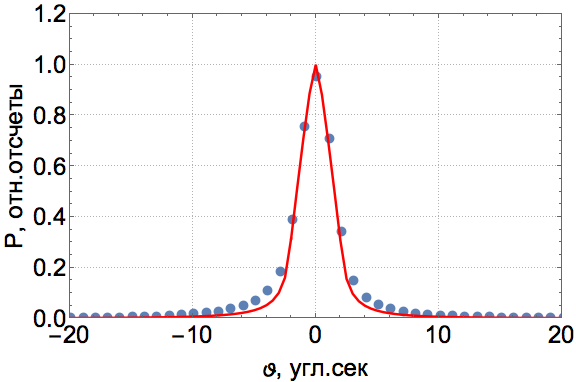
\includegraphics[width=0.45\textwidth]{images/non_disspers_20_40.png}\label{fig:f1}}
  \hfill
  \subfloat[]{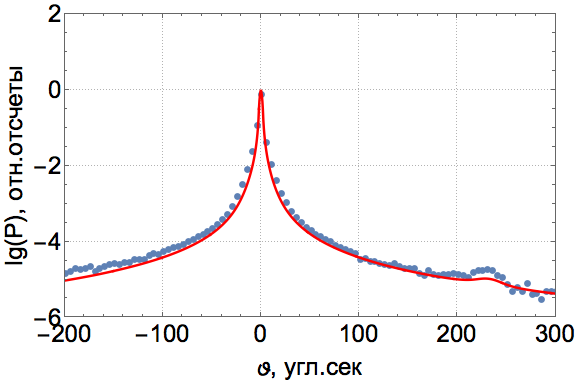
\includegraphics[width=0.45\textwidth]{images/non_disspers_20_40_log.png}\label{fig:non_disspers_kdo_1}}
  \hfill
  \subfloat[]{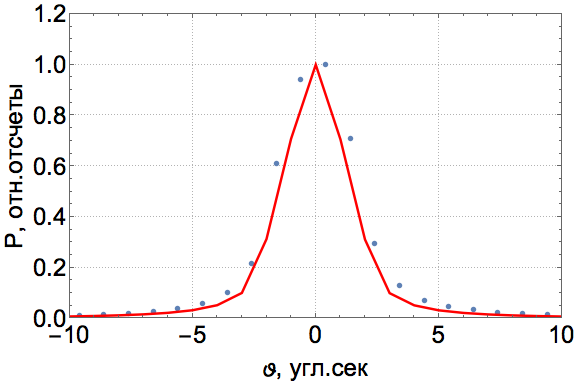
\includegraphics[width=0.45\textwidth]{images/non_disspers_300_200.png}\label{fig:f2}}
  \hfill
  \subfloat[]{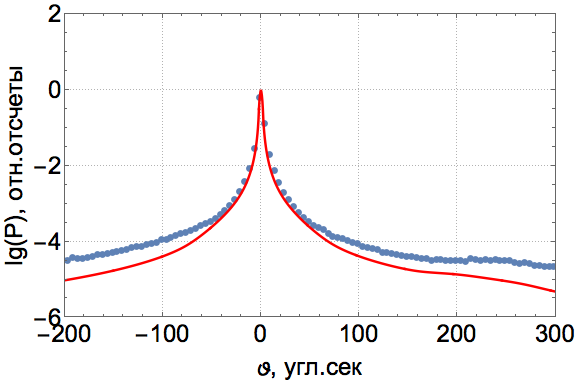
\includegraphics[width=0.45\textwidth]{images/non_disspers_300_200_log.png}\label{fig:f2}}
  \caption{Двухкристальная КДО для схемы с установленным кристаллом монохроматором Si(220) и образцом  Si(220). Расстояние до щелевых устройств
  составляет $L_1= 570 $мм, $L_2 = 1005$ мм. Линейный размер источника $\delta = 0.1$ мм. (красная линия) - расчет, (синие точки) - эксперимент
  для размеров щелевых устройств (a) $S_1 = 20 $ мкм; $ S_2 = 40$ мкм, (b) $S_1 = 20 $ мкм; $ S_2 = 40$ мкм,
  (c) $S_1 = 300 $ мкм; $ S_2 = 200$ мкм, (d) $S_1 = 300 $ мкм; $ S_2 = 200$ мкм}
  \label{ris:non_disspers_kdo}
\end{figure}

На рис. \ref{fig:non_disspers_kdo_1} видно, что наряду с главным пиком, соответствующим $k_{\alpha1}$ лиинии
излучения, на которую настроен монохроматор, присутствует вклад от соседней характеристической линии
 $k_{\alpha2}$. Впервые, на это свойство двухкристальных КДО, получаемы в бездисперсионной
схеме, в случае использования рентгеновской трубки было указано авторами работы \cite{chuev2008}
